% !TEX root = ../main.tex
\section{Числові характеристики випадкових величин}
Закон розподілу випадкової величини в будь-якому вигляді (ряд розподілу для ДВВ, щільність розподілу для НВВ, функція розподілу в загальному випадку)
повністю задає випадкову величину. Однак в прикладних задачах іноді достатньо мати лише деяке сумарне уявлення про деякі характерні невипадкові риси розподілу.

\subsection{Математичне сподівання}
\begin{definition}\index{математичне сподівання}
    \emph{Математичним сподіванням} $\E\xi$ випадкової величини називається значення
    інтеграла Стілтьєса
    \begin{equation}\label{eq:e_xi}
        \E\xi = \int\limits_{-\infty}^{+\infty} x dF_\xi(x) = \begin{cases}
            \sum\limits_{k=1}^{n(\infty)} x_k \P\left\{\xi = x_k\right\}, & \xi \text{ --- ДВВ} \\
            \int\limits_{-\infty}^{+\infty} x f_\xi(x)dx, & \xi \text{ --- НВВ}
        \end{cases}
    \end{equation}
\end{definition}
Інтеграл або ряд \eqref{eq:e_xi} має збігатися \emph{абсолютно}, інакше кажуть, що
випадкова величина не має математичного сподівання. Ця вимога пояснюється тим, що, наприклад, у випадку ДВВ зі зліченною множиною значень не має бути різниці,
в якому порядку додавати всі значення.
\begin{example}\index{розподіл!Коші}
    НВВ, розподілена за законом Коші з щільністю $f_\xi(x) = \frac{1}{\pi (1+x^2)}$
    не має математичного сподівання, бо інтеграл $\frac{1}{\pi}\int\limits_{-\infty}^{+\infty} \frac{x}{1+x^2}dx$ 
    розбіжний.
\end{example}
Математичне сподівання характеризує середнє значення випадкової величини. Наприклад,
якщо ДВВ набуває скінченну кількість значень з однаковими ймовірностями, то математичним сподіванням є просто середнім арифметичним усіх цих значень.
Фізична інтерпретація --- центр мас системи точок $\left\{x_1, x_2, ..., x_n,...\right\}$ з масами $\left\{p_1, p_2, ..., p_n, ...\right\}$ (ДВВ) або стрижня,
розподіл маси в якому задано функцією щільності (НВВ).

\vspace{0.5em}
\noindent \textbf{Властивості математичного сподівання:}
\begin{enumerate}
    \item Математичне сподівання константи --- сама константа, оскільки
    її можна інтерпретувати як ДВВ, що приймає єдине значення з ймовірністю $1$:
    $c = const, \E c = c$.
    \item $\E \left(c\cdot\xi\right) = c\cdot \E\xi$ --- це властивість рядів та інтегралів.
    \item $\E\left( \xi_1 + \xi_2\right) = \E\xi_1 + \E\xi_2$.
    \begin{proof}[Доведення для ДВВ]
        $\P\left\{\xi_1 = x_k\right\} = p_k$, $\P\left\{\xi_2 = y_j\right\} = p_j$, $\P\left\{\xi_1 + \xi_2 = x_k + y_j\right\} = p_{kj}$.
        В цих позначеннях
        $\E\left( \xi_1 + \xi_2\right) = \sum\limits_k \sum\limits_j (x_k+y_j) p_{kj} =
        \sum\limits_k x_k \sum\limits_j p_{kj} + \sum\limits_j y_j \sum\limits_k p_{kj} = \sum\limits_k x_k p_k + \sum\limits_j y_j p_j = \E\xi_1 + \E\xi_2$.
    \end{proof}
\suspend{enumerate}
\begin{definition}\index{випадкова величина!незалежні величини}
    Дві випадкові величини $\xi_1$ та $\xi_2$, задані на одному ймовірнісному просторі, називаються \emph{незалежними}, якщо
    події $A=\left\{\omega : \; \xi_1(\omega) < x\right\}$ та
    $B=\left\{\omega : \; \xi_2(\omega) < y\right\}$ є незалежними для всіх $x, y \in \mathbb{R}$.
\end{definition}
\resume{enumerate}
    \item Якщо $\xi_1$ та $\xi_2$ незалежні, то $\E\xi_1\xi_2 = \E\xi_1 \cdot \E\xi_2$.
    \begin{proof}[Доведення для ДВВ]
        Позначимо $p_{kj} = \P\left\{\xi_1 = x_k, \xi_2 = y_j\right\}$.
        
        $\E\xi_1\xi_2 = \sum\limits_k \sum\limits_j x_k y_j p_{kj} = \sum\limits_k \sum\limits_j x_k y_j p_k p_j = \left( \sum\limits_k x_k p_k\right)\cdot \left( \sum\limits_j y_j p_j\right) = \E\xi_1 \cdot \E\xi_2$.
    \end{proof}
\end{enumerate}
\begin{remark}
    Властивості 3 та 4 для НВВ буде доведено в темі <<Функції випадкових аргументів>> (ст. \pageref{proof:expectation}).
\end{remark}

\begin{example}
    \begin{enumerate}
        \item Обчислити математичне сподівання двох ДВВ:
        
        \begin{center}
            \begin{tabular}{c c}
                \begin{tabular}{|c|c|c|}
                    \hline
                    $\xi_1$ & $-1$ & $1$ \\ 
                    \hline
                    $p$ & $1/2$ & $1/2$ \\
                    \hline
                \end{tabular} &
                \begin{tabular}{|c|c|c|}
                    \hline
                    $\xi_2$ & $-100$ & $100$ \\ 
                    \hline
                    $p$ & $1/2$ & $1/2$ \\
                    \hline
                \end{tabular}
            \end{tabular}
        \end{center}
        $\E\xi_1 = -1\cdot \frac{1}{2} + 1\cdot \frac{1}{2} = 0, \E\xi_2 = -100\cdot \frac{1}{2} + 100\cdot \frac{1}{2} = 0$.
        
        Цей приклад показує, що попри однакове значення математичного сподівання, можливі значення цих ДВВ знаходяться на різній відстані від нього,
        тому знання математичного сподівання ще не дає повного уявлення про закон розподілу випадкової величини.        
        \item Обчислити математичне сподівання НВВ, розподіленої за законом Сімпсона.\index{розподіл!Сімпсона}

        \begin{tabular}{c c}
            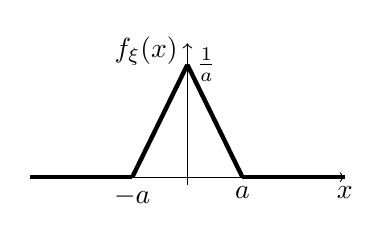
\begin{tikzpicture}[baseline={(current bounding box.center)}, yscale=1]
                \pgfmathsetmacro{\a}{0.7}
                \draw [->] (-2, 0) -- (2, 0);
                \draw [->] (0, -0.1) -- (0, 1.7);
                \draw [ultra thick] (-2, 0) -- (-\a, 0);
                \draw [ultra thick] (\a, 0) -- (2, 0);
                \draw [ultra thick] (-\a, 0) -- (0, 1/\a);
                \draw [ultra thick] (\a, 0) -- (0, 1/\a);
                \node [below] at (2, 0) {$x$};
                \node [left] at (0, 1.6) {$f_\xi(x)$};
                \node [below] at (\a, 0) {$a$};
                \node [below] at (-\a, 0) {$-a$};
                \node [right] at (0, 1/\a) {$\frac{1}{a}$};
            \end{tikzpicture} &
            $f_\xi(x) = \begin{cases}
                \frac{1}{a} \left(1 - \frac{|x|}{a}\right), & |x| \leq a \\
                0, & |x| > a
            \end{cases} \;(a>0)$
        \end{tabular}
        
        $\E\xi = \int\limits_{-\infty}^{+\infty} x f_\xi(x)dx = \int\limits_{-a}^a \frac{x}{a}\left(1 - \frac{|x|}{a}\right)dx = 0$, 
        оскільки інтегрується непарна функція по симетричному проміжку.
    \end{enumerate}
\end{example}

\subsection{Дисперсія}
Як було показано, випадкові величини можуть мати однакові математичні сподівання, але відхилення значень цих випадкових величин
від нього може бути різним. Треба ввести ще одну числову характеристику,
що описуватиме це.
\begin{definition}\index{дисперсія}
    \emph{Дисперсією} випадкової величини називається 
    \begin{equation}\label{eq:d_xi}
        \D\xi = \E\left(\xi-\E\xi\right)^2 = \int\limits_{-\infty}^{+\infty} \left(x-\E\xi\right)^2 dF_\xi(x) = \begin{cases}
            \sum\limits_{k=1}^{n(\infty)} \left(x_k-\E\xi\right)^2 \P\left\{\xi = x_k\right\}, & \xi \text{ --- ДВВ} \\
            \int\limits_{-\infty}^{+\infty} \left(x-\E\xi\right)^2 f_\xi(x)dx, & \xi \text{ --- НВВ}
        \end{cases}
    \end{equation}
\end{definition}
Дисперсія --- характеристика розсіювання випадкової величини навколо свого математичного сподівання.
Фізична інтерпретація --- момент інерції маси системи точок або стрижня (як і у випадку інтерпретації математичного сподівання)
відносно свого центру мас.
\begin{remark}
    Дисперсія визначена тоді і тільки тоді, коли математичне сподівання існує та є скінченним.
    Оскільки в \eqref{eq:d_xi} і члени ряду, і підінтегральна функція є невід'ємними, то
    дисперсія може бути або скінченною, або рівною $+\infty$.
\end{remark}

\begin{example}
    \begin{enumerate}
        \item Обчислити дисперсії двох ДВВ:
        
        \begin{center}
            \begin{tabular}{c c}
                \begin{tabular}{|c|c|c|}
                    \hline
                    $\xi_1$ & $-1$ & $1$ \\ 
                    \hline
                    $p$ & $1/2$ & $1/2$ \\
                    \hline
                \end{tabular} &
                \begin{tabular}{|c|c|c|}
                    \hline
                    $\xi_2$ & $-100$ & $100$ \\ 
                    \hline
                    $p$ & $1/2$ & $1/2$ \\
                    \hline
                \end{tabular}
            \end{tabular}
        \end{center}
        
        $\D\xi_1 = (-1)^2\cdot \frac{1}{2} + 1^2\cdot \frac{1}{2} = 1, \D\xi_2 = (-100)^2\cdot \frac{1}{2} + 100^2\cdot \frac{1}{2} = 10000$.
        Тут вже видно різницю між двома випадковими величинами: значення $\xi_2$ розташовані далеко від математичного сподівання і тому дисперсія більша, ніж у $\xi_1$.
        \item Обчислити дисперсію НВВ, розподіленої за законом Сімпсона.
        
        Відповідна щільність розподілу має вигляд $f_\xi(x) = \begin{cases}
            \frac{1}{a} \left(1 - \frac{|x|}{a}\right), & |x| \leq a \\
            0, & |x| > a
        \end{cases}$.
        Математичне сподівання вже було обчислено, воно рівне 0. Тому $\D\xi = \int\limits_{-\infty}^{+\infty} \left(x-\E\xi\right)^2 f_\xi(x)dx =
        \int\limits_{-a}^a \frac{x^2}{a}\left(1 - \frac{|x|}{a}\right)dx = \frac{2}{a}\int\limits_0^a {x^2}\left(1 - \frac{x}{a}\right)dx =
        \frac{2}{a}\cdot \left( \frac{x^3}{3} - \frac{x^4}{4a}\right)\Bigr\vert_0^a = \frac{2}{a} \cdot \left( \frac{a^3}{3} - \frac{a^3}{4}\right) = \frac{a^2}{6}$.
    \end{enumerate}
\end{example}

\noindent \textbf{Властивості дисперсії:}
\begin{enumerate}\index{середньоквадратичне відхилення}
    \item $\D\xi \geq 0$, $\sqrt{\D\xi} = \sigma_\xi$ --- \emph{середньоквадратичне (стандартне) відхилення}.
    \item $\D\xi = 0 \Leftrightarrow \xi = const$.
    \begin{proof}
        В одну сторону: $\D c = \E(c - \E c)^2 = \E(c - c)^2 = 0$. В іншу: якщо $\xi$ --- ДВВ,
        то з $\D\xi = 0$ випливає, що $\left(x_k-\E\xi\right)^2 = 0$ для всіх $k$,
        тому для всіх $k$ $x_k = \E \xi$ --- $\xi$ приймає лише одну значення.
        Для НВВ аналогічно випливає, що $\left(x-\E\xi\right)^2 f_\xi(x) \equiv 0$. Оскільки $\left(x-\E\xi\right)^2$
        рівне $0$ лише в точці $x=\E\xi$, то $f_\xi(x)$ може бути відмінним від 0 лише в цій точці. Але тоді $f_\xi(x)$ не може бути щільністю,
        тому що площа під кривою розподілу має бути рівною 1. Це свідчить про дискретність $\xi$,
        і тому за вже доведеним $\xi$ приймає лише одне значення.
    \end{proof}
    \item Для обчислення дисперсії більш зручною є наступна формула:

    $\D\xi = \E(\xi^2 - 2\xi \E\xi +(\E\xi)^2) = \E\xi^2 - 2(\E\xi)^2 + (\E\xi)^2 = \E\xi^2 - (\E\xi)^2$. 
    \item Для сталої $c$: $\D(c\cdot \xi) = c^2\cdot \D\xi$, оскільки $\D(c\cdot \xi) = \E\left(c\cdot\xi-\E(c\cdot\xi\right))^2 = \E\left(c\cdot\xi - c\cdot \E\xi\right)^2 = c^2 \cdot \E\left(\xi-\E\xi\right)^2 = c^2 \cdot \D\xi$.
    \item Для сталої $c$: $\D(\xi + c) = \E(\xi + c - \E(\xi + c))^2 = \E(\xi + c - \E\xi - \E c) = \E(\xi - \E\xi)^2 = \D\xi$.
\suspend{enumerate}
\begin{definition}\index{випадкова величина!центрована}
    \emph{Центрованою} випадковою величиною, що відповідає випадковій величині $\xi$, називається 
    випадкова величина $\mathring{\xi} = \xi - \E\xi$. Для неї $\E\mathring{\xi} = 0$ та 
    $\E\mathring{\xi^2} = \D\xi$.
\end{definition}
\resume{enumerate}
    \item Якщо випадкові величини $\xi_1$ та $\xi_2$ --- незалежні, то
    $\D\left(\xi_1 + \xi_2\right) = \D\xi_1 + \D\xi_2$.
    \begin{proof}
        $\D\left(\xi_1 + \xi_2\right) = \E((\xi_1 + \xi_2) - \E(\xi_1 + \xi_2))^2 = \E(\mathring{\xi}_1 + \mathring{\xi}_2)^2 =
        \E\mathring{\xi}_1^2 + 2\E\mathring{\xi}_1\mathring{\xi}_2 + \E\mathring{\xi}_2^2 = 
        \E\mathring{\xi}_1^2 + 2\E\mathring{\xi}_1 \E\mathring{\xi}_2 + \E\mathring{\xi}_2^2 =
        \E\mathring{\xi}_1^2 + \E\mathring{\xi}_2^2 = \D\xi_1 + \D\xi_2$.
    \end{proof}
\end{enumerate}

\subsection{Моменти випадкової величини}
\begin{definition}\index{момент!початковий}
    \emph{Початковим моментом k-того порядку} ($k \in \mathbb{N}$) ВВ $\xi$ називається
    математичне сподівання $k$-того степеня $\xi$:
    \begin{equation}\label{eq:e_alpha_k}
        \alpha_k = \E\xi^k = \int\limits_{-\infty}^{+\infty} x^k dF_\xi(x) = \begin{cases}
            \sum\limits_{m=1}^{n(\infty)} x_m^k \P\left\{\xi = x_m\right\}, & \xi \text{ --- ДВВ} \\
            \int\limits_{-\infty}^{+\infty} x^k f_\xi(x)dx, & \xi \text{ --- НВВ}
        \end{cases}
    \end{equation}
\end{definition}
\begin{definition}\index{момент!центральний}
    \emph{Центральним моментом k-того порядку} ($k \in \mathbb{N}$) ВВ $\xi$ називається
    \begin{equation}\label{eq:d_beta_k}
        \beta_k = \E\mathring{\xi}^k = \E\left(\xi-\E\xi\right)^k = \int\limits_{-\infty}^{+\infty} \left(x-\E\xi\right)^k dF_\xi(x) = \begin{cases}
            \sum\limits_{m=1}^{n(\infty)} \left(x_m-\E\xi\right)^k \P\left\{\xi = x_m\right\}, & \xi \text{ --- ДВВ} \\
            \int\limits_{-\infty}^{+\infty} \left(x-\E\xi\right)^k f_\xi(x)dx, & \xi \text{ --- НВВ}
        \end{cases}
    \end{equation}
\end{definition}
Математичне сподівання є початковим моментом першого порядку, а дисперсія --- центральним моментом другого порядку.
Узагальненням формули для дисперсії
$\D\xi = \beta_2 = \E\xi^2 - (\E\xi)^2 = \alpha_2 - \alpha_1^2$ є наступна формула,
що дозволяє виразити будь-який центральний момент через початкові моменти:
\begin{equation}
    \beta_k = \E\left(\xi-\E\xi\right)^k = \E\left( \sum\limits_{j=0}^k C_k^j \xi^j (-1)^{k-j} (\E\xi)^{k-j}\right) =
\sum\limits_{j=0}^k (-1)^{k-j} C_k^j \E\xi^j (\E\xi)^{k-j}
\end{equation}
\begin{exercise}
    Виразити через початкові моменти $\beta_3$ та $\beta_4$.
\end{exercise}
Розглядаються також \emph{абсолютні початкові моменти}\index{момент!початковий!абсолютний} $\E\vert \xi \vert ^k$, 
\emph{абсолютні центральні моменти}\index{момент!центральний!абсолютний} $\E\vert \xi - \E\xi \vert ^k$
та \emph{факторіальні моменти}\index{момент!факторіальний} $\gamma_k = \E\left( \xi (\xi - 1) ... (\xi - k + 1)\right)$.
\begin{remark}
    Якщо за змістом задачі випадкова величина має якісь одиниці вимірювання (наприклад, метри чи кілограми),
    то моменти $k$-того порядку мають відповідний порядок одиниць вимірювання.
    Наприклад, якщо деяка випадкова величина задає похибку вимірювання в міліметрах,
    то математичне сподівання теж буде у міліметрах, а дисперсія --- в квадратних міліметрах
    (але середньоквадратичне відхилення --- просто у міліметрах).
\end{remark}


\subsection{Мода та медіана випадкової величини}
\begin{definition}\index{мода}
    \emph{Модою} $\Mo\xi$ називається абсциса точки максимуму щільності 
    розподілу у випадку НВВ та значення, ймовірність 
    появи якого є найбільшим, у випадку ДВВ.

    \emph{Унімодальний закон} --- такий, що має лише одну моду. 
    \emph{Полімодальний закон} --- такий, що має декілька мод.
    \emph{Антимодальний закон} --- такий, що не має моди.
\end{definition}
\begin{definition}\index{медіана}
    \emph{Медіаною} $\Me\xi$ НВВ $\xi$ називається така точка $x_0$, для якої 
    $\P\left\{\xi < x_0\right\} = \P\left\{\xi \geq x_0\right\} 
    = \frac{1}{2} \Leftrightarrow F_\xi(x_0) = \frac{1}{2}$.
    Для ДВВ $\xi$ медіаною є така точка $x_0$, для якої одночасно
    виконуються нерівності $\P\left\{\xi < x_0\right\} \geq \frac{1}{2}$ та
    $\P\left\{\xi \geq x_0\right\} \geq \frac{1}{2}$.
    Медіана є окремим випадком \emph{квантиля}.
\end{definition}
\begin{definition}\index{квантиль}
    Точка $x_0$ називається \emph{квантилем q-го порядку}, якщо $F_\xi(x_0) = q$ 
    для НВВ $\xi$ або $F_\xi(x_0) \geq q$ та $F_\xi(x_0) \geq 1-q$ для ДВВ.
\end{definition}
\begin{example}
    Знайти моду та медіану НВВ, розподіленої за законом Релея.\index{розподіл!Релея}
    
    \begin{tabular}{c c}
        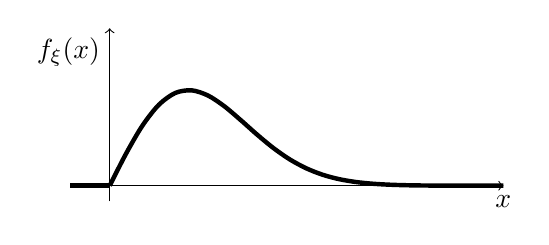
\begin{tikzpicture}[baseline={(current bounding box.center)}, yscale=2]
            \pgfmathsetmacro{\s}{1}
            \draw [->] (-0.5, 0) -- (5, 0);
            \draw [->] (0, -0.1) -- (0, 1);
            \node [below] at (5, 0) {$x$};
            \node [below left] at (0, 1) {$f_\xi(x)$};
            \draw [domain=0:5, smooth, variable = \x, ultra thick] plot ({\x}, {((\x/(\s^2)) * exp(-(\x)^2/(2*\s^2))});
            \draw [ultra thick] (-0.5, 0) -- (0, 0);
        \end{tikzpicture} &
        $f_\xi(x) = \begin{cases}
            \frac{x}{\sigma^2} e^{-\frac{x^2}{2\sigma^2}}, & x \geq 0 \\
            0, & x < 0
        \end{cases} (\sigma > 0)$ 
    \end{tabular}

    Для визначення моди знайдемо максимум $f_\xi(x)$ при $x\geq 0$.
    $f'_\xi(x) = \frac{\sigma^2 - x^2}{\sigma^4} e^{-\frac{x^2}{2\sigma^2}} = 0$ при $x=\sigma$.
    $f''_\xi(x) = \left( -\frac{3x}{\sigma^4} + \frac{x^3}{\sigma^6}\right) e^{-\frac{x^2}{2\sigma^2}}$,
    $f''_\xi(\sigma) = -\frac{2}{\sigma^3} e^{-\frac{1}{2}} < 0$. Отже, в точці $x=\sigma$ дійсно максимум $f_\xi(x)$, тому $\Mo\xi = \sigma$.

    Медіану знайдемо з рівності $\P\left\{\xi < x_0\right\} = 0.5$. $\P\left\{\xi < x_0\right\} = \int\limits_{-\infty}^{x_0}f_\xi(x)dx = 
    \int\limits_0^{x_0} \frac{x}{\sigma^2} e^{-\frac{x^2}{2\sigma^2}} dx = 1 - e^{-\frac{x_0^2}{2\sigma^2}}$.
    З рівняння $1 - e^{-\frac{x_0^2}{2\sigma^2}} = 0.5$ знаходимо $x_0 = \Me\xi = \sigma \sqrt{2\ln{2}}$.
\end{example}

\subsection{Асиметрія та ексцес випадкової величини}
\begin{definition}\index{асиметрія}
    \emph{Асиметрією} випадкової величини $\As\xi$ називається безрозмірна 
    числова характеристика, що дорівнює $\frac{\beta_3}{\sigma_\xi^3} = 
    \frac{\E(\xi - \E\xi)^3}{(\D\xi)^{3/2}}$. 
    Ця характеристика показує порушення чи наявність симетрії кривої розподілу відносно математичного сподівання.
\end{definition}
\begin{center}
    \begin{tabular}{c c c}
        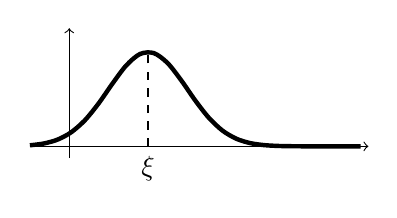
\begin{tikzpicture}[yscale = 1.5]
            \draw [->] (-0.5, 0) -- (3.8, 0);
            \draw [->] (0, -0.1) -- (0, 1);
            \draw [domain=-0.5:3.7, smooth, variable = \x, ultra thick] plot ({\x}, {0.797884560803 * exp(-2*(\x-1)^2)});
            \draw [dashed] (1, 0) -- (1, 0.797884560803);
            \node [below] at (1, 0) {$\E\xi$};
        \end{tikzpicture} &
        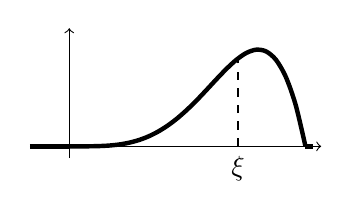
\begin{tikzpicture}[yscale = 1.5]
            \draw [->] (-0.5, 0) -- (3.2, 0);
            \draw [->] (0, -0.1) -- (0, 1);
            \draw [ultra thick] (-0.5, 0) -- (0, 0);
            \draw [ultra thick] (3, 0) -- (3.1, 0);
            \draw [domain=0:3, smooth, variable = \x, ultra thick] plot ({\x}, {10 * (\x/3)^4 * (1-(\x/3))});
            \draw [dashed] (2.1428, 0) -- (2.1428, 0.744);
            \node [below] at (2.1428, 0) {$\E\xi$};
        \end{tikzpicture} &
        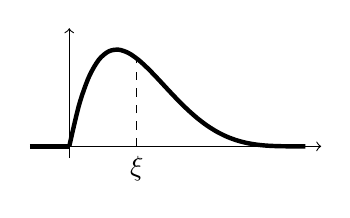
\begin{tikzpicture}[yscale = 1.5]
            \draw [->] (-0.5, 0) -- (3.2, 0);
            \draw [->] (0, -0.1) -- (0, 1);
            \draw [ultra thick] (-0.5, 0) -- (0, 0);
            \draw [domain=0:3, smooth, variable = \x, ultra thick] plot ({\x}, {10 * (\x/3) * (1-(\x/3))^4});
            \draw [dashed] (0.8571, 0) -- (0.8571, 0.744);
            \node [below] at (0.8571, 0) {$\E\xi$};
        \end{tikzpicture} \\
        $\As\xi = 0$ & $\As\xi < 0$ & $\As\xi > 0$ 
    \end{tabular}
\end{center}

\begin{definition}\index{ексцес}
    \emph{Ексцесом} випадкової величини $\Ex\xi$ називається безрозмірна 
    числова характеристика, що дорівнює $\Ex\xi = \frac{\beta_4}{\sigma_\xi^4} - 3 = 
    \frac{\E(\xi - \E\xi)^4}{(\D\xi)^{2}} - 3$.
    Ця характеристика показує, наскільки швидко крива розподілу 
    прямує до точки максимуму.
\end{definition}
\begin{center}
    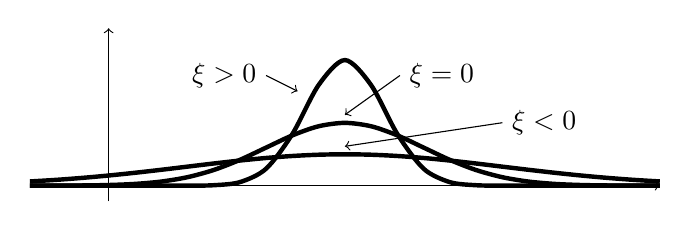
\begin{tikzpicture}[yscale = 2]
        \draw [->] (-1, 0) -- (7, 0);
        \draw [->] (0, -0.1) -- (0, 1);
        \draw [domain=-1:7, smooth, variable = \x, ultra thick] plot ({\x}, {0.398942280401 * exp(-(\x-3)^2/2)});
        \draw [domain=-1:7, smooth, variable = \x, ultra thick] plot ({\x}, {0.797884560803 * exp(-2*(\x-3)^2)});
        \draw [domain=-1:7, smooth, variable = \x, ultra thick] plot ({\x}, {0.199471140201 * exp(-(\x-3)^2/8)});
        \draw [->] (2, 0.7) -- (2.4, 0.6);
        \node [left] at (2, 0.7) {$\Ex\xi > 0$};
        \draw [->] (3.7, 0.7) -- (3, 0.45);
        \node [right] at (3.7, 0.7) {$\Ex\xi = 0$};
        \draw [->] (5, 0.4) -- (3, 0.25);
        \node [right] at (5, 0.4) {$\Ex\xi < 0$};
    \end{tikzpicture}
\end{center}

\subsection{Генератриса (твірна функція) ДВВ}
\begin{definition}\index{генератриса (твірна функція)}
    Нехай $\xi$ --- ДВВ, що приймає цілі невід'ємні значення. 
    \emph{Генератрисою (твірною функцією)} цієї ДВВ називається функція комплексного аргументу
    \begin{equation}\label{eq:gen_func}
        G_\xi(z) = \sum\limits_{k=0}^{\infty} \P\left\{\xi = k\right\} z^k
    \end{equation}
\end{definition}
\noindent \textbf{Властивості генератриси:}
\begin{enumerate}
    \item Відповідний ряд рівномірно збігається принаймні в колі $|z|\leq 1$.
    \begin{proof}
        Випливає з того, що $\left| \sum\limits_{k=0}^{\infty} \P\left\{\xi = k\right\} z^k \right| \leq \sum\limits_{k=0}^{\infty} \P\left\{\xi = k\right\} = 1$.
    \end{proof}
    \item Генератриса --- аналітична функція в колі $|z|\leq 1$ (як наслідок властивості 1).
    \item За генератрисою можна відновити розподіл $\xi$:
    $\P\left\{\xi = k\right\} = \frac{1}{k!}\cdot G_\xi^{(k)}(0)$.
    \item За допомогою генератриси можна знайти факторіальні моменти $\xi$.
    \begin{proof}
        За означенням факторіальний момент $\gamma_m = \E\left( \xi (\xi - 1) ... (\xi - m + 1)\right)$.
        Для ДВВ, що розглядаються, він рівний $\sum\limits_{k=0}^{\infty} k(k-1)(k-2)...(k-m+1) \P\left\{\xi = k\right\}$.
        З іншого боку, $G'_\xi(z) = \sum\limits_{k=0}^{\infty} k \P\left\{\xi = k\right\} z^{k-1}$,
        $G''_\xi(z) = \sum\limits_{k=0}^{\infty} k(k-1) \P\left\{\xi = k\right\} z^{k-2}$ і так далі,
        $G^{(m)}_\xi(z) = \sum\limits_{k=0}^{\infty} k(k-1)(k-2)...(k-m+1) \P\left\{\xi = k\right\} z^{k-m}$.
        Отже, $\gamma_m = G^{(m)}_\xi(1)$.
    \end{proof}
\end{enumerate}
Як наслідок властивості 4, можна також знайти математичне сподівання та дисперсію.
Факторіальний та початковий моменти першого порядку збігаються, тому $\E\xi = G'_\xi(1)$.
Дисперсію знайдемо за допомогою другого факторіального моменту: $\gamma_2 = \E\left( \xi (\xi - 1)\right) = \E\xi^2 - \E\xi = G''_\xi(1)$,
звідки $\E\xi^2 = G''_\xi(1) + G'_\xi(1)$. 
Отже, $\D\xi = \E\xi^2 - (\E\xi)^2 = G''_\xi(1) + G'_\xi(1) - \left( G'_\xi(1)\right)^2$.
\begin{exercise}
    Виразити через похідні генератриси центральні моменти 3-го та 4-го порядків.
\end{exercise}